
%(BEGIN_QUESTION)
% Copyright 2010, Tony R. Kuphaldt, released under the Creative Commons Attribution License (v 1.0)
% This means you may do almost anything with this work of mine, so long as you give me proper credit

Dette termoelementet er installert feil:

$$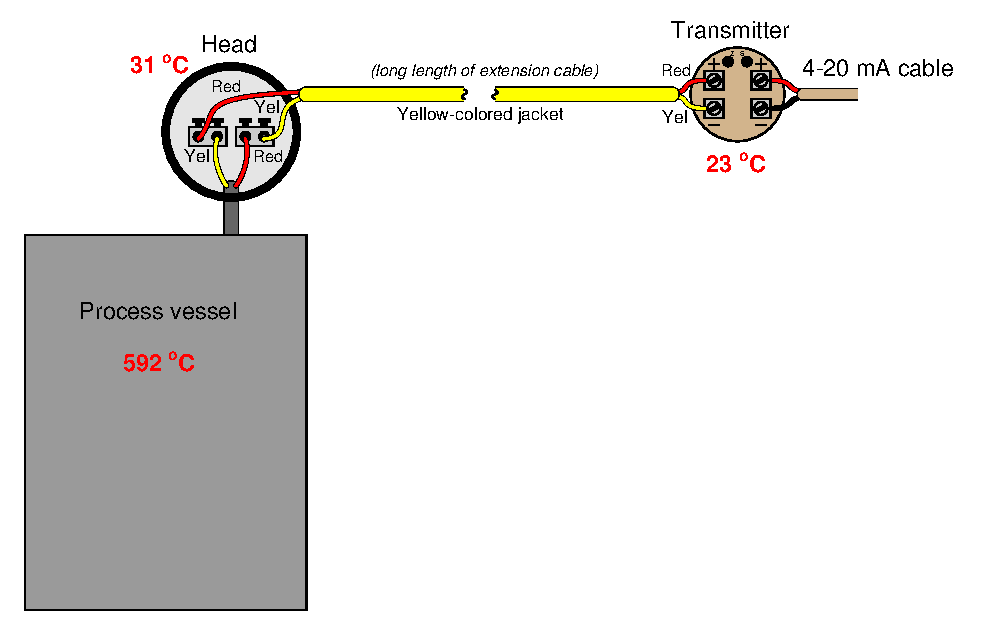
\includegraphics[width=15.5cm]{i00633x01.eps}$$

Identifiser hva slags feil dette er, og beregn deretter millivoltspenningen ved skruterminalene til temperaturtransmitteren gitt temperaturene som er vist. Etterpå beregner du temperaturen transmitteren vil tolke når kaldskjøtkompensering (CJC) er aktivert.

\underbar{file i00633no}
%(END_QUESTION)





%(BEGIN_ANSWER)

Forlengelseslederen er koblet "baklengs" til termoelementet. Gul skal kobles til gul, og rød til rød.

\vskip 10pt

Slik de {\it fire} skjøtenes spenninger virker sammen, er det best å tegne kretsen med hver skjøt tydelig merket med polaritet. Da ser du at prosesskjøten og referanseskjøten (i transmitteren) virker i samme retning, mens de to skjøtene i hodet virker mot de to første (men i samme retning som hverandre). Formelen for å beregne spenningen ved transmitterens skruterminaler blir da:

$$V_{terminals} = V_{592^oC} + V_{23^oC} - V_{31^oC} - V_{31^oC}$$

$$V_{terminals} = 24.565 \hbox{ mV} + 0.919 \hbox{ mV} - 1.244 \hbox{ mV} - 1.244 \hbox{ mV}$$

$$V_{terminals} = 22.996 \hbox{ mV}$$

Hvis transmitteren har CJC aktivert, vil den {\it legge til} 0.919 mV for å kompensere for referanseskjøten, slik at tolket spenning (måleskjøtspenning) blir 23.915 mV. Dette tilsvarer 577 $^{o}$C, som er betydelig lavere enn den faktiske prosesstemperaturen.

%(END_ANSWER)





%(BEGIN_NOTES)

%INDEX% Måling, temperatur: tolkning av termoelement-millivolt

%(END_NOTES)
